\chapter{Konzeption \& Entwurf}
\label{cha:konzeption}
In diesem Kapitel wird das anfängliche Spielkonzept mit Hilfe von Mock-Ups visualisiert und evaluiert. Anschließend wird in Kapitel \ref{sec:konzeption:konzept} das umgesetzte Spielkonzept vorgestellt.

\section{Mock-Ups}
\label{sec:konzeption:prototyping:mockups}
Die ursprüngliche Idee des Spiels war ein Spielverlauf von oben nach unten, wodurch die beiden Spieler einen Abgrund (\textit{Abyss}) hinabspringen müssen, um einen Endgegner zu bekämpfen. Dabei springen beide Spieler durchgehend und um mit der Device-Motion die Richtung zu ändern (ähnlich zu \href{https://play.google.com/store/apps/details?id=com.lima.doodlejump&hl=de}{\textit{Doodle Jump}}). Jedoch sind durch dieses Leveldesign die Möglichkeiten der Levelgestaltung, als auch die Bewegungsfreiheit der Spieler stark eingeschränkt.
\begin{figure}[H]
    \begin{center}
      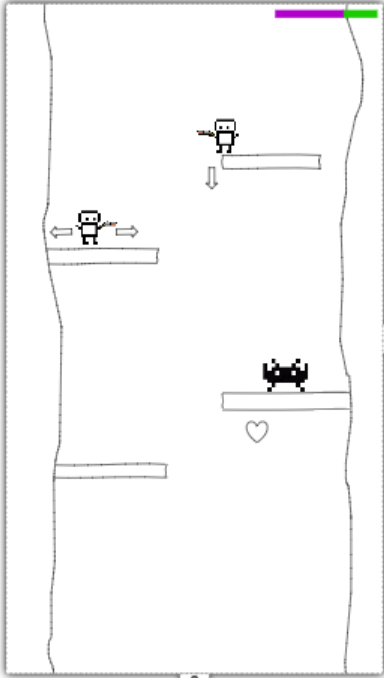
\includegraphics[width=.22\linewidth]{img/konzeption/Jump}
      \caption{Steuerung}
      \label{fig:konzeption:prototyping:jump}
    \end{center}
\end{figure}


Zusätzlich sollten Waffen in dem Spiel eingesetzt werden können, jedoch sind die Steuerungsmöglichkeiten an einem Smartphone mit den Möglichkeiten zu springen, schießen und bewegen des Spielers stark eingeschränkt und fehleranfällig.

\begin{figure}[H]
    \begin{center}
      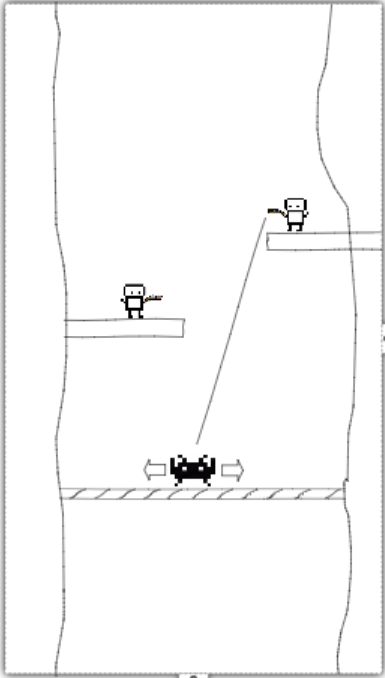
\includegraphics[width=.22\linewidth]{img/konzepFtion/Fight}
      \caption{Waffen}
      \label{fig:konzeption:prototyping:fight}
    \end{center}
\end{figure}


Zur Beendigung des Levels müssen beide Spieler das Ende erreichen um anschließend einen Endgegner zu besiegen. Wie in Kapitel \ref{sec:implementierung:probleme} erklärt, ist das designen von Assets anspruchsvoll und zeitaufwendig.
\begin{figure}[H]
    \begin{center}
      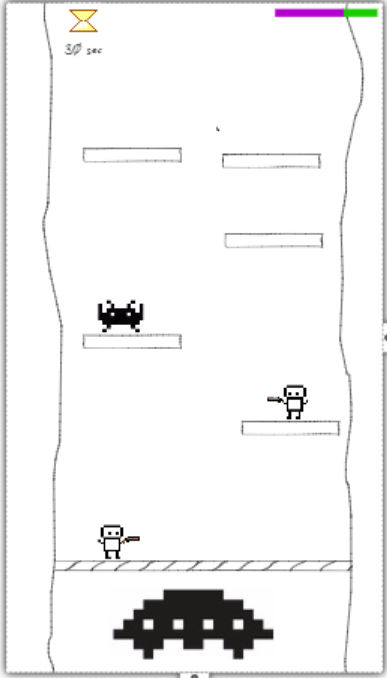
\includegraphics[width=.22\linewidth]{img/konzeption/EndBoss}
      \caption{Endboss}
      \label{fig:konzeption:prototyping:endboss}
    \end{center}
\end{figure}

\section{Spielkonzept}
\label{sec:konzeption:konzept}
In diesem Kapitel werden Spieleigenschaften, der Aufbau der Level und der Funktionsumfang der verschiedenen Spielobjekte erläutert. Die Ansicht der Spiels ist zweidimensional, daher werden die Level stets von der Seite dargestellt.

\subsection{Level}
\label{sec:konzeption:konzept:level}
 Die jeweiligen Level des Spiels beschäftigen sich mit einem eigenen Thema (mit eigenem Licht, Musik und Umfeld). Um ein Zusammenspielen der Spieler zu erzwingen müssen beide Spieler das Level beenden. Erst wenn beide Spieler das Ziel erreichen, ist das Level beendet. Damit das Level beendet werden kann, müssen im Laufe des Spiels zwei Schlüssel eingesammelt, die es erst ermöglichen das Ziel in Form einer Truhe zu erreichen. Spieler können anfangs nur das erste Level spielen, erst nach Beendigung des Levels wird das darauffolgende Level freigeschalten und somit spielbar. 

\subsection{Spielobjekte}
\label{sec:konzeption:konzept:spielobjekte}
Um das Spiel für den Spieler attraktiver zu gestalten werden verschiedene Spielobjekte verwendet, die das Spiel interessanter und abwechslungsreicher gestalten sollen. Diese Spielobjekte können den Spieler einen Vorteil verschaffen (\textit{Power-Up}), Schaden zufügen (\textit{Gegner}) oder transportieren (\textit{Plattform}). Zusätzlich gibt es Spielobjekte, die das Passieren eines bestimmten Spielers verhindern (\textit{Barriere}) und somit einen Weg erzwingt, der sich von dem des anderen Spielers unterscheidet. Um entfernte oder abgeschnittene Spielbereiche zu erreichen und das Spiel somit komplexer zu gestalten werden \textit{Portale} verwendet, die den Spieler zu einem zugehörigen Portal transportieren. Wie bereits in Kapitel \ref{sec:konzeption:konzept:level} erwähnt existieren genau zwei \textit{Schlüssel}, die zum Beendigen des Levels benötigt werden. Das Ziel des Spiels hat die Form einer \textit{Truhe}, die von beiden Spielern erreicht werden muss.

\subsection{Spieler}
\label{sec:konzeption:konzept:spieler}
Da das Spiel für genau zwei Spieler ausgelegt ist, werden für die gleiche Spielfigur zwei verschiedene Farben verwendet um die Spieler darzustellen und zu unterscheiden. Die Handlungsmöglichkeiten der Spieler sind auf Laufen (nach rechts oder links) und Springen beschränkt. Spieler sind zusätzlich in der Lage Wall-Jumps (abspringen an einer Wand) zu vollziehen.

Kommt ein Spieler mit einem Hindernis in Kontakt verliert der jeweilige Spieler je nach Hindernis ein Teil seines Lebens. In Spielen wie \textit{Super Mario} stirbt der Spieler sofort nach Kontakt mit einem Hindernis. Sollte ein Spieler im Laufe eines Levels sterben, müssen beide Spieler das Level von vorne beginnen.

Um das Zusammenspielen in bestimmten Level zu erzwingen und um das Spiel um eine Feature zu erweitern, erhält der zurückbleibende Spieler schaden, falls der Abstand zwischen Ihm und dem Mitspieler zu groß wird.

\subsection{Steuerung}
\label{sec:konzeption:konzept:steuerung}
Um die Nutzung der Anwendung übersichtlich zu halten wird die Spielsteuerung möglichst simpel gestalten. Die Bewegung des Spielers von links nach rechts wird am Smartphone durch die Device-Motion ermöglicht (Neigung des Smartphones). Um die Touchgesten einfach zu halten, kann der Spieler mit einem Klick springen. Gleitet der Spieler eine Wand herunter, kann zu diesem Moment der Sprung verwendet werden, um von der Wand abzuspringen und so einen Wall-Jump zu vollziehen. 

Am Computer wird für die Steuerung die links bzw. rechts Taste verwendet. Zum Springen muss die Leertaste betätigt werden.


% Abschnitt: Layout
\section{Layout}
\label{sec:konzeption:layout}
Das Spiel soll bis zum Spielstart einen geregelten Ablauf haben. Die Spieler haben nach dem Spielstart die Möglichkeit sich mit ihrem Account anzumelden oder zu registrieren. Anschließend wird das Hauptmenü der Anwendung angezeigt. Dort hat man die Möglichkeit einen Raum zu erstellen oder einem bereits bestehenden Raum beizutreten. Erstellt ein Spieler einen Raum muss er noch das Level auswählen, das gespielt werden soll. Anschließend wartet der Spieler, der den Raum erstellt hat, auf den anderen Spieler und kann das Spiel im ausgewählten Level starten. Die Abbildung \ref{fig:konzeption:layout:menu} zeigt diesen Menu-Ablauf bis zum Starten des Spiels. Jeder Zustand repräsentiert dabei einen Screen der Anwendung. 

\begin{figure}[H]
    \begin{center}
      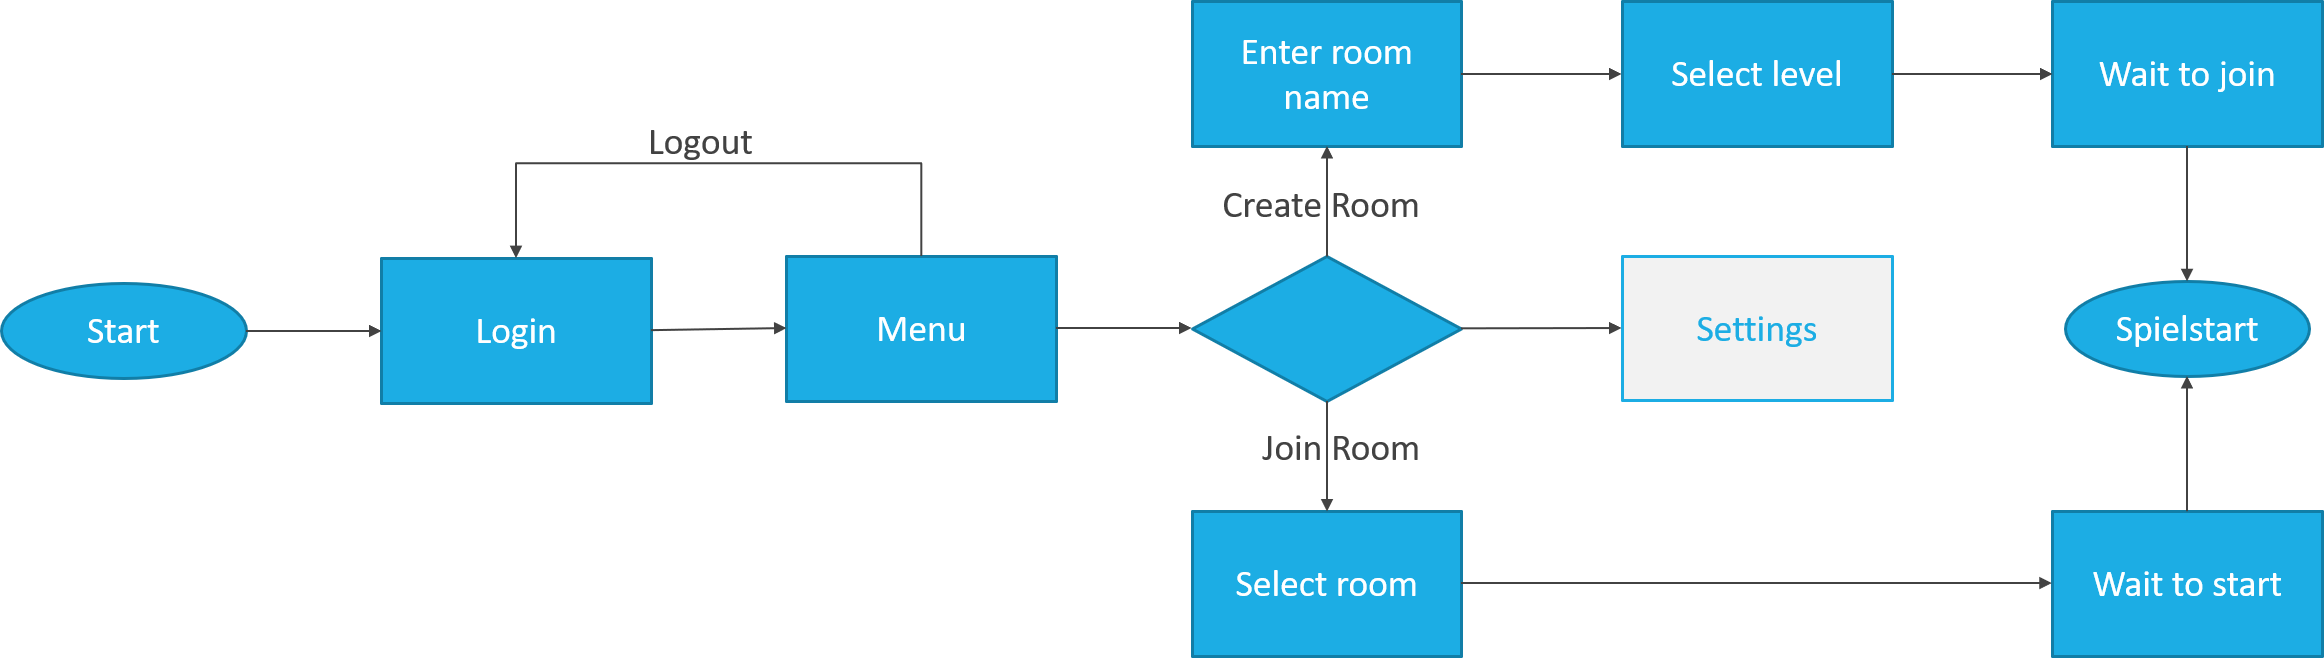
\includegraphics[width=\linewidth]{img/konzeption/Spielablauf2}
      \caption{Menüauswahl}
      \label{fig:konzeption:layout:menu}
    \end{center}
\end{figure}

Neben dem Erstellen bzw. Beitreten eines Raums kann man im Hauptmenü zusätzlich die Musiklautstärke verändern. Dabei kann die Hintergrundmusik, die In-Game-Geräusche und die Klick-Laustärke des Button-Feedbacks eingestellt werden.